% Options for packages loaded elsewhere
\PassOptionsToPackage{unicode}{hyperref}
\PassOptionsToPackage{hyphens}{url}
\PassOptionsToPackage{dvipsnames,svgnames,x11names}{xcolor}
%
\documentclass[
  singlecolumn]{report}

\usepackage{amsmath,amssymb}
\usepackage{iftex}
\ifPDFTeX
  \usepackage[T1]{fontenc}
  \usepackage[utf8]{inputenc}
  \usepackage{textcomp} % provide euro and other symbols
\else % if luatex or xetex
  \usepackage{unicode-math}
  \defaultfontfeatures{Scale=MatchLowercase}
  \defaultfontfeatures[\rmfamily]{Ligatures=TeX,Scale=1}
\fi
\usepackage[]{libertinus}
\ifPDFTeX\else  
    % xetex/luatex font selection
\fi
% Use upquote if available, for straight quotes in verbatim environments
\IfFileExists{upquote.sty}{\usepackage{upquote}}{}
\IfFileExists{microtype.sty}{% use microtype if available
  \usepackage[]{microtype}
  \UseMicrotypeSet[protrusion]{basicmath} % disable protrusion for tt fonts
}{}
\makeatletter
\@ifundefined{KOMAClassName}{% if non-KOMA class
  \IfFileExists{parskip.sty}{%
    \usepackage{parskip}
  }{% else
    \setlength{\parindent}{0pt}
    \setlength{\parskip}{6pt plus 2pt minus 1pt}}
}{% if KOMA class
  \KOMAoptions{parskip=half}}
\makeatother
\usepackage{xcolor}
\usepackage[top=30mm,left=20mm,heightrounded]{geometry}
\setlength{\emergencystretch}{3em} % prevent overfull lines
\setcounter{secnumdepth}{-\maxdimen} % remove section numbering
% Make \paragraph and \subparagraph free-standing
\ifx\paragraph\undefined\else
  \let\oldparagraph\paragraph
  \renewcommand{\paragraph}[1]{\oldparagraph{#1}\mbox{}}
\fi
\ifx\subparagraph\undefined\else
  \let\oldsubparagraph\subparagraph
  \renewcommand{\subparagraph}[1]{\oldsubparagraph{#1}\mbox{}}
\fi


\providecommand{\tightlist}{%
  \setlength{\itemsep}{0pt}\setlength{\parskip}{0pt}}\usepackage{longtable,booktabs,array}
\usepackage{calc} % for calculating minipage widths
% Correct order of tables after \paragraph or \subparagraph
\usepackage{etoolbox}
\makeatletter
\patchcmd\longtable{\par}{\if@noskipsec\mbox{}\fi\par}{}{}
\makeatother
% Allow footnotes in longtable head/foot
\IfFileExists{footnotehyper.sty}{\usepackage{footnotehyper}}{\usepackage{footnote}}
\makesavenoteenv{longtable}
\usepackage{graphicx}
\makeatletter
\def\maxwidth{\ifdim\Gin@nat@width>\linewidth\linewidth\else\Gin@nat@width\fi}
\def\maxheight{\ifdim\Gin@nat@height>\textheight\textheight\else\Gin@nat@height\fi}
\makeatother
% Scale images if necessary, so that they will not overflow the page
% margins by default, and it is still possible to overwrite the defaults
% using explicit options in \includegraphics[width, height, ...]{}
\setkeys{Gin}{width=\maxwidth,height=\maxheight,keepaspectratio}
% Set default figure placement to htbp
\makeatletter
\def\fps@figure{htbp}
\makeatother

\usepackage{booktabs}
\usepackage{longtable}
\usepackage{array}
\usepackage{multirow}
\usepackage{wrapfig}
\usepackage{float}
\usepackage{colortbl}
\usepackage{pdflscape}
\usepackage{tabu}
\usepackage{threeparttable}
\usepackage{threeparttablex}
\usepackage[normalem]{ulem}
\usepackage{makecell}
\usepackage{xcolor}
\usepackage{cancel}
\makeatletter
\makeatother
\makeatletter
\makeatother
\makeatletter
\@ifpackageloaded{caption}{}{\usepackage{caption}}
\AtBeginDocument{%
\ifdefined\contentsname
  \renewcommand*\contentsname{Table of contents}
\else
  \newcommand\contentsname{Table of contents}
\fi
\ifdefined\listfigurename
  \renewcommand*\listfigurename{List of Figures}
\else
  \newcommand\listfigurename{List of Figures}
\fi
\ifdefined\listtablename
  \renewcommand*\listtablename{List of Tables}
\else
  \newcommand\listtablename{List of Tables}
\fi
\ifdefined\figurename
  \renewcommand*\figurename{Figure}
\else
  \newcommand\figurename{Figure}
\fi
\ifdefined\tablename
  \renewcommand*\tablename{Table}
\else
  \newcommand\tablename{Table}
\fi
}
\@ifpackageloaded{float}{}{\usepackage{float}}
\floatstyle{ruled}
\@ifundefined{c@chapter}{\newfloat{codelisting}{h}{lop}}{\newfloat{codelisting}{h}{lop}[chapter]}
\floatname{codelisting}{Listing}
\newcommand*\listoflistings{\listof{codelisting}{List of Listings}}
\makeatother
\makeatletter
\@ifpackageloaded{caption}{}{\usepackage{caption}}
\@ifpackageloaded{subcaption}{}{\usepackage{subcaption}}
\makeatother
\makeatletter
\@ifpackageloaded{tcolorbox}{}{\usepackage[skins,breakable]{tcolorbox}}
\makeatother
\makeatletter
\@ifundefined{shadecolor}{\definecolor{shadecolor}{rgb}{.97, .97, .97}}
\makeatother
\makeatletter
\makeatother
\makeatletter
\makeatother
\ifLuaTeX
  \usepackage{selnolig}  % disable illegal ligatures
\fi
\IfFileExists{bookmark.sty}{\usepackage{bookmark}}{\usepackage{hyperref}}
\IfFileExists{xurl.sty}{\usepackage{xurl}}{} % add URL line breaks if available
\urlstyle{same} % disable monospaced font for URLs
\hypersetup{
  pdftitle={Test},
  pdfauthor={Joseph A. Bulbulia},
  pdfkeywords={Author order TBA.},
  colorlinks=true,
  linkcolor={blue},
  filecolor={Maroon},
  citecolor={Blue},
  urlcolor={Blue},
  pdfcreator={LaTeX via pandoc}}

\title{Test}
\usepackage{etoolbox}
\makeatletter
\providecommand{\subtitle}[1]{% add subtitle to \maketitle
  \apptocmd{\@title}{\par {\large #1 \par}}{}{}
}
\makeatother
\subtitle{An outcome-wide study}
\author{Joseph A. Bulbulia}
\date{}

\begin{document}
\maketitle
\begin{abstract}
Test
\end{abstract}
\ifdefined\Shaded\renewenvironment{Shaded}{\begin{tcolorbox}[frame hidden, boxrule=0pt, interior hidden, sharp corners, borderline west={3pt}{0pt}{shadecolor}, breakable, enhanced]}{\end{tcolorbox}}\fi

\listoffigures
\listoftables
\hypertarget{test}{%
\section{Test}\label{test}}

\[Y(a)\cancel{\coprod} A|L\]

\hypertarget{dag}{%
\section{Dag}\label{dag}}

\begin{figure}

{\centering 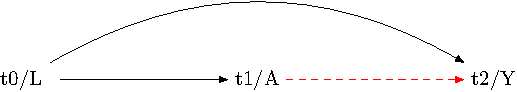
\includegraphics[width=1\textwidth,height=\textheight]{test-latex_files/figure-pdf/fig-dag-common-cause-1.pdf}

}

\caption{\label{fig-dag-common-cause}Counfounding by common cause.}

\end{figure}

\hypertarget{tbl-consistency}{}
\begin{longtable}[]{@{}lll@{}}
\caption{\label{tbl-consistency}Causal Consistency}\tabularnewline
\toprule\noalign{}
Group & Exposure (A=1) & No Exposure (A=0) \\
\midrule\noalign{}
\endfirsthead
\toprule\noalign{}
Group & Exposure (A=1) & No Exposure (A=0) \\
\midrule\noalign{}
\endhead
\bottomrule\noalign{}
\endlastfoot
Y(1) & Observable & Counterfactual \\
Y(0) & Counterfactual & Observable \\
\end{longtable}

Note Figure~\ref{fig-dag-common-cause2} Here I offer a comprehensive
tutorial that showcases the practical utility of temporally organised
causal diagrams.\footnote{It is tempting to call temporally organised
  causal diagrammes ``temporal action graphs'' - or ``TAGs.'' However,
  we do not need more jargon.} Temporally organised causal diagrams are
ordinary directed acyclic graphs (DAGs) in which the spatial structure
of the graph is designed to reflected the temporal order of assumed
causality. We may think of such graphs as temporally conscientious
causal DAGS.\footnote{Note that the contrast may be between different
  levels of a multinomial categorical or continuous indicator, in which
  case we would define the levels to contrast as \(A = a\) and
  \(A = a*\) \begin{align}
  ATE = E(Y(a) - Y(a*))
  \end{align}}

\hypertarget{dags}{%
\section{Dags}\label{dags}}

\begin{figure}

{\centering \includegraphics[width=0.8\textwidth,height=\textheight]{test-latex_files/figure-pdf/fig-dag-common-cause2-1.pdf}

}

\caption{\label{fig-dag-common-cause2}Counfounding by common cause.}

\end{figure}

\begin{figure}

{\centering 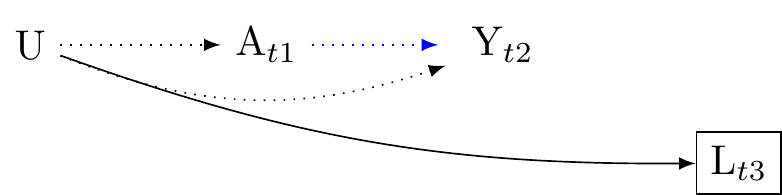
\includegraphics[width=0.8\textwidth,height=\textheight]{test-latex_files/figure-pdf/fig-dag-descendent-solution-2-1.pdf}

}

\caption{\label{fig-dag-descendent-solution-2}Solution: note that
conditioning on a confounder that occurs after the exposure and outcome
addresses the problem of unmeasured confounding. The dotted paths denote
that the effect of U on A and Y is partially adjusted by conditioning on
L, even though L occurs after the outcome. The dotted blue path suggest
suppressing of the biased relationship between A and Y under the null. A
genetic factor that affects the exposure and the outcome early in life,
and that also expresses a measured indicator late in life, might
constitute an example for which post-outcome confounding control might
be possible.}

\end{figure}

\begin{figure}

{\centering 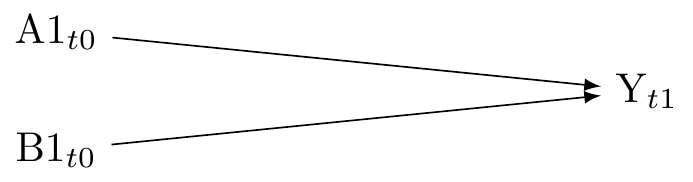
\includegraphics[width=0.8\textwidth,height=\textheight]{test-latex_files/figure-pdf/fig-dag-interaction-1.pdf}

}

\caption{\label{fig-dag-interaction}Causal interaction: if two exposures
are causally independent of each other, we may wish to estimate their
individual and joint effects on Y, where the counterfactual outcome is
Y(a,b) and there is evidence for additive or subadditive interaction if
E{[}Y(1,1) - Y(0,1) - Y(1,0) + Y(0,0){]} ≠ 0}

\end{figure}



\end{document}
